\documentclass[12pt,addpoints]{exam}
\usepackage[utf8]{inputenc}
\usepackage{lastpage}
\usepackage{amsmath}
\usepackage{amsfonts}
\usepackage{amssymb}
\usepackage{enumerate}
\usepackage{mdframed}
\usepackage{array}
\usepackage{graphics}
\usepackage{graphicx}
\usepackage{listings}
\usepackage{tikz}
\usetikzlibrary{arrows}
\usepackage{algpseudocode}

% Paramètres globaux
\bonuspointpoints{point \emph{bonus}}{points \emph{boni}}
\parindent 0cm
\hqword{Question}
\hpword{Sur}
\hsword{Note}
\htword{Total}

% Solutions
\printanswers

% En-tête et pieds de page
\headrule
\cfoot{\thepage /\pageref{LastPage}}
\lhead{INF5071 --- Infographie}
\rhead{Automne 2016}
\newcommand{\headrulewidth}{0.4pt}
\newcommand{\footrulewidth}{0.4pt}

% Algorithmes
\algrenewcommand\algorithmicwhile{\textbf{tant que}}
\algrenewcommand\algorithmicfunction{\textbf{fonction}}
\algrenewcommand\algorithmicend{\textbf{fin}}
\algrenewcommand\algorithmicdo{\textbf{faire}}
\algrenewcommand\algorithmicfor{\textbf{pour}}
\algrenewcommand\algorithmicif{\textbf{si}}
\algrenewcommand\algorithmicelse{\textbf{sinon}}
\algrenewcommand\algorithmicthen{\textbf{alors}}
\algrenewcommand\algorithmicreturn{\textbf{retourner}}
\algrenewcommand\algorithmicrepeat{\textbf{faire}}
\algrenewcommand\algorithmicuntil{\textbf{tant que}}
\newcommand{\enteteproc}[2]{\vskip\baselineskip \hspace*{\fill} \algorithmicprocedure~\Call{#1}{#2} \hspace*{\fill} \vskip\baselineskip}
\newcommand{\entetefunc}[3]{\vskip\baselineskip \hspace*{\fill} \algorithmicfunction~\Call{#1}{#2} : #3 \hspace*{\fill} \vskip\baselineskip}

% Code
\lstset{
  literate={é}{{\'e}}1
           {è}{{\`e}}1
           {ê}{{\^e}}1
           {î}{{\^i}}1
           {à}{{\`a}}1
           {É}{{\'E}}1,
  basicstyle=\footnotesize\ttfamily,
  keywordstyle=\bfseries\color{green!70!black},
  identifierstyle=\color{blue},
  commentstyle=\ttfamily\color{red!70!black}\emph,
  stringstyle=\bfseries\color{orange},
  showstringspaces=false,
  language=python,
  breaklines=true
}

% Raccourcis
\newcommand{\bigo}{\mathcal{O}}
\newcommand{\N}{\mathbb{N}}
\newcommand{\R}{\mathbb{R}}

\begin{document}
	
\ifprintanswers
  \vskip 1.2cm
  \centerline{\large\underline{\textbf{Solution du devoir 1}}}
  \vskip 0.5cm
  \begin{mdframed} \begin{center}
  \textbf{Auteur : Alexandre Blondin Massé} \\
  \end{center} \end{mdframed}
  \vskip 0.5cm
\else
  \vskip 1.2cm
  \centerline{\large\underline{\textbf{Devoir 1}}}
  \centerline{\small (à remettre au plus tard le 19 octobre, à 16h00)}
  \centerline{\small (en classe ou dans la chute du département d'informatique, située au PK-4150)}
  \vskip 1.2cm
Le devoir doit être rédigé \textbf{individuellement} et à l'\textbf{ordinateur} (il est cependant permis de remettre des annexes avec des \textbf{schémas dessinés} manuellement). Vous devez \textbf{justifier} chacune de vos réponses. Tout retard entraînera une pénalité de \textbf{20\%} par jour ouvrable.
\fi

\ifprintanswers
\else
\begin{center} \gradetable[h] \end{center}
\fi

\begin{questions}

% Projection isométrique
\question
Supposons qu'une application graphique utilise des images de dimensions $64 \times 32$ pixels$^2$ pour représenter des tuiles en \emph{projection isométrique} (dans le dessin ci-bas, un exemple d'image contenant une tuile est identifié par un rectangle bleu).
\begin{parts}
  \part[15] Expliquez comment calculer la position du coin supérieur gauche d'une tuile $10 \times 10$ qu'on place dans une grille indexée comme l'illustre la grille ci-bas~:
\begin{center} 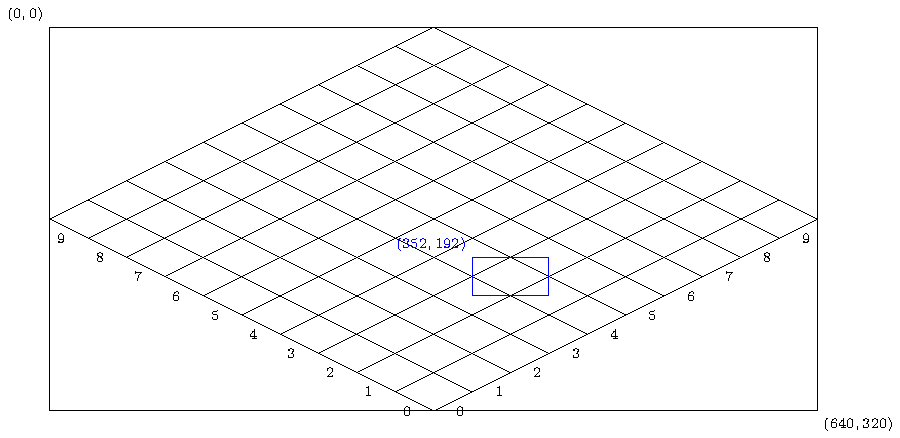
\includegraphics{images/isometrique.pdf} \end{center}
Autrement dit, donnez le pseudocode d'une fonction
\entetefunc{CoinSupGauche}{$i,j$ : indices}{point}
qui retourne la position que devrait occuper le coin supérieur gauche du rectangle contenant la tuile aux indices $i$ et $j$. Par exemple, on s'attend à ce que l'appel $\Call{CoinSupGauche}{4,2}$ retourne la valeur $(352,192)$ (voir le rectangle bleu dans l'image ci-haut).
	\newpage
	\begin{solution}
		\begin{algorithmic}[1]
		\Function{CoinSupGauche}{$i,j$ : indices} : {point}
		\State $x\gets 288$
		\State $y\gets 288$
	
		\State $x\gets x + (i * 32)$
		\State $y\gets y - (i * 16)$
	
		\State $x\gets x - (j * 32)$
		\State $y\gets y - (j * 16)$
		
		\State \textbf{return} $(x,y)$
		\EndFunction
		\end{algorithmic}
	\end{solution}

  \part[10] Dans la question ci-bas, nous avons supposé que toutes les tuiles se trouvaient à la même hauteur. Supposons que nous souhaitions également supporter la possibilité d'afficher des tuiles plus hautes que d'autres. En utilisant des notions d'algèbres linéaire et vectorielle, expliquez de quelle façon vous traiteriez cette situation et montrez en particulier que certaines tuiles à des hauteurs différentes pourraient apparaître exactement au même endroit.
	\begin{solution}
		Pour traiter la situation, on pourrait ajouter une 3e composante à la grille; appelons-là \emph{K}. Elle servirait à spécifier la hauteur d'une tuile. Elle agirait sur la tuile en décrémentant les composantes \emph{Y} des points qui constituent la tuile et la façon suivante :
\[
\begin{bmatrix}
    x_{1}       & y_{1} \\
    x_{2}       & y_{2} \\
    x_{3}       & y_{3} \\
    x_{4}       & y_{4} \\
\end{bmatrix}
-
\begin{bmatrix}
    0       & K \\
    0       & K\\
    0       & K\\
    0       & K\\
\end{bmatrix}
=
\begin{bmatrix}
    x_{1}       & y_{1} - K \\
    x_{2}       & y_{2} - K\\
    x_{3}       & y_{3} - K\\
    x_{4}       & y_{4} - K\\
\end{bmatrix}
\]
Alors, pour 
\[
	k \in \N \implies k \mod 32 = 0
\]
la tuile pourrait se situer exactement au même endroit qu'une des tuiles sans hauteur. Voici un example : 
\[
k = 32, i = 0, j = 0
\]
\[
\begin{bmatrix}
    320       & 320 \\
    352       & 304 \\
    320       & 288 \\
    288       & 304 \\
\end{bmatrix}
-
\begin{bmatrix}
    0       & 32 \\
    0       & 32\\
    0       & 32\\
    0       & 32\\
\end{bmatrix}
=
\begin{bmatrix}
    320       & 288 \\
    352       & 272\\
    320       & 256\\
    288       & 272\\
\end{bmatrix}
\]
ce qui correspond au coordonnées des points de la tuile située en
\[
k = 0, i = 1, j = 1
\]
	\end{solution}
  \bonuspart[5] Le concepteur principal d'un jeu appelé \emph{Super Hexagon} est auteur d'un autre jeu qui exploite le fait que différentes tuiles à des hauteurs différentes apparaissent au même endroit. Quel est le nom de ce jeu et qui en est l'auteur ?
	\begin{solution}
		Le jeu se nomme \emph{Hexagon} et son créateur est \emph{Terry Cavanagh}.
	\end{solution}
\end{parts}

% Génération procédurale
\question[20]
Supposez que les services suivants sont disponibles pour manipuler des maillages~:
\begin{itemize}
  \item $M \gets \Call{MaillageVide}$ construit un maillage vide et le stocke dans la variable $M$.
  \item $M.\Call{AjouterSommet}{p}$ ajoute un sommet dans le maillage $M$ et dont les coordonnées sont données par le point $p$.
  \item $M.\Call{AjouterArete}{p_1,p_2}$ ajoute une arête entre les sommets $p_1$ et $p_2$ dans le maillage $M$. Si un ou les deux sommets n'existent pas dans la structure, une erreur est signalée.
  \item $M.\Call{AjouterFace}{P}$ ajoute une face dont les sommets sont donnés par la liste $P$. Ces sommets doivent être énumérés dans l'ordre antihoraire lorsqu'on regarde vers l'\emph{extérieur} de la face. De plus, s'il n'y a pas d'arêtes entre deux sommets consécutifs, une erreur est signalée.
\end{itemize}

Donnez le \textbf{pseudocode} d'une fonction dont l'en-tête est
\entetefunc{Grille}{$m,n$ : entiers positifs, $d,e$ : réels}{maillage}
et qui retourne un maillage modélisant une grille de $m$ carrés par $n$ carrés, dont l'épaisseur est donnée par $e$ et la distance entre les carrés de la grille est donnée par $d$. Autrement dit, si vous implémentiez votre fonction dans un script Blender et que vous utilisiez les paramètres $m = 3$, $n = 4$, $e = 0.1$ et $d = 1.0$, alors vous vous attendriez à obtenir un maillage similaire à celui illustré dans l'image ci-bas.

\textbf{Attention !} La topologie de votre maillage doit être bien définie. Autrement dit, aucune erreur ne doit être signalée (vous devez donc d'abord ajouter les sommets, ensuite les arêtes, puis finalement les faces) et vous devez vous assurer que c'est le côté \emph{visible} des faces (c'est-à-dire vers l'extérieur) qui est décrit en sens antihoraire.

\textbf{Note~:} Vous pouvez utiliser la notation $[p_1,p_2,p_3,p_4]$ pour dénoter une liste qui contient les quatre points $p_1$, $p_2$, $p_3$ et $p_4$ (autrement dit, vous pouvez utiliser des crochets pour dénoter des listes). Aussi, bien que ce ne soit pas demandé dans la question, n'hésitez pas à vérifier votre stratégie en l'implémentant comme un script Blender !

\begin{center} 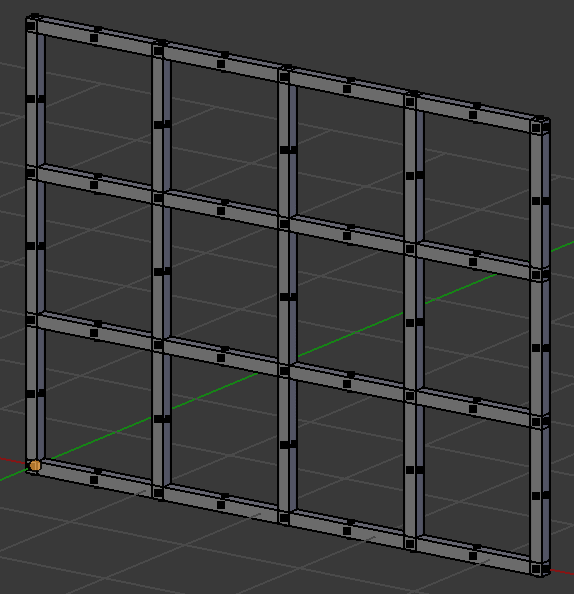
\includegraphics[width=.45\linewidth]{images/grille-3d.png} \end{center}

Voici une vue de face d'une portion de la grille avec les dimensions correspondantes~:

\begin{center} 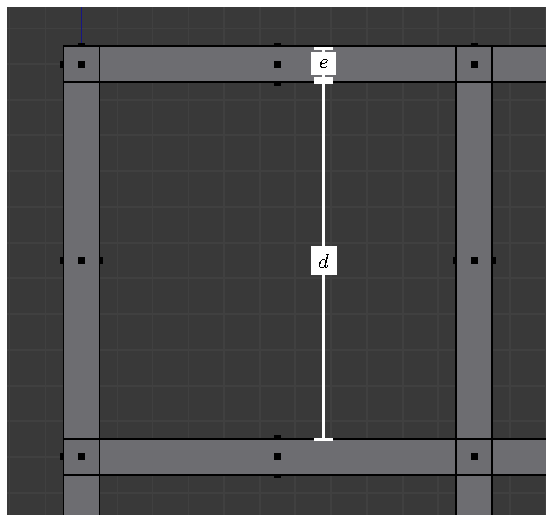
\includegraphics{images/grille.pdf} \end{center}
\newpage
\begin{solution}
	\begin{algorithmic}[1]
	\Procedure{Rectangle}{$m$: maillage, $x,y,x,h,l$: réels, $inclinaison$: chaîne, $flipVertex$=Faux: booléen}
	\If {$inclinaison = "FACE"$}
		\State $s1\gets (x,y,z)$
	 	\State $s2\gets (x + l,y,z)$
		\State $s3\gets (x + l,y,z - h)$
		\State $s4\gets (x,y,z - h)$
	\ElsIf {$inclinaison = "COUCHE"$}
	   	\State $s1\gets (x,y,z)$
	 	\State $s2\gets (x,y + h,z)$
		\State $s3\gets (x + l,y + h,z)$
		\State $s4\gets (x + l,y,z)$
	\ElsIf {$inclinaison = "COTE"$}
	   	\State $s1\gets (x,y,z)$
	 	\State $s2\gets (x,y + l,z)$
		\State $s3\gets (x,y + l,z - h)$
		\State $s4\gets (x,y,z - h)$
	\EndIf
	
	\State \Call{m.AjouterSommet}{s1}
	\State \Call{m.AjouterSommet}{s2}
	\State \Call{m.AjouterSommet}{s3}
	\State \Call{m.AjouterSommet}{s4}

	\State \Call{m.AjouterArrete}{s1,s2}
	\State \Call{m.AjouterArrete}{s2,s3}
	\State \Call{m.AjouterArrete}{s3,s4}
	\State \Call{m.AjouterArrete}{s4,s1}

	\State $P\gets [s1,s2,s3,s4]$

	\If {$flipVertex$}
		\State \Call{P.Reverse}{}
	\EndIf

	\State \Call{m.AjouterFace}{P}

	\EndProcedure
\newpage
	\Procedure{Tige}{$m$: maillage, $x,y,z,e,d$: réels,  $sens$: chaîne,  $inclinaison$: chaîne, $flipVertex$=Faux: booléen}
	\If {$sens = "DROITE"$}
		\State \Call{Rectangle}{m, x, y, z, e, e, inclinaison, flipVertex}
		\State \Call{Rectangle}{m, x + e, y, z, e, d, inclinaison, flipVertex}
		\State \Call{Rectangle}{m, x + e + d, y, z, e, e, inclinaison, flipVertex}
	\EndIf

	\If {$sens = "BAS"$}
		\State \Call{Rectangle}{m, x, y, z, e, e, inclinaison, flipVertex}
		\State \Call{Rectangle}{m, x, y, z - e, e, d, inclinaison, flipVertex}
		\State \Call{Rectangle}{m, x, y, z - e - d, e, e, inclinaison, flipVertex}
	\EndIf

	\EndProcedure
\newline
	\Procedure{Cadre}{$m$: maillage, $x,y,x,e,d$: réels, $flipVertex$=Faux: booléen}
	\State \Call{Tige}{m, x, y, z, e, d, "DROITE", "FACE", flipVertex}
	\State \Call{Tige}{m, x + e + d, y, z, e, d, "BAS", "FACE", flipVertex}
	\State \Call{Tige}{m, x, y, z - e - d, e, d, "DROITE", "FACE", flipVertex}
	\State \Call{Tige}{m, x, y, z, e, d, "BAS", "FACE", flipVertex}
	\EndProcedure
\newline
	\Procedure{Contour}{$m$: maillage, $x,y,x,e,d$: réels}
	\State \Call{Tige}{m, x, y, z, e, d, "DROITE", "COUCHE"}
	\State \Call{Tige}{m, x + 2 * e + d, y, z, e, d, "BAS", "COTE"}
	\State \Call{Tige}{m, x, y, z - 2 * e - d, e, d, "DROITE", "COUCHE", Vrai}
	\State \Call{Tige}{m, x, y, z, e, d, "BAS", "COTE", Vrai}
	\EndProcedure
\newline
	\Procedure{Carre}{$m$: maillage, $x,y,x,e,d$: réels}
	\State \Call {Cadre}{m, x, y, z, e, d}
	\State \Call {Cadre}{m, x, y + e, z, e, d, Vrai}
	\State \Call {Contour}{m, x, y, z, e, d}
	
	\State \Call{Rectangle}{m, x + e, y, z - e, e, d, "COUCHE", Vrai}
	\State \Call{Rectangle}{m, x + e + d, y, z - e, d, e, "COTE", Vrai}
	\State \Call{Rectangle}{m, x + e, y, z - e - d, e, d, "COUCHE"}
	\State \Call{Rectangle}{m, x + e, y, z - e, d, e, "COTE"}
	
	\EndProcedure
\newpage
	\Procedure{Grille}{$m,n$: entiers positifs, $d,e$ : réels}{maillage}
	\State  $maillage\gets \Call{MaillageVide}{}$
	\State  $x\gets 0.0$
	\State  $y\gets 0.0$
	\State  $z\gets 0.0$

	\For{$i$ entre 0 et $m$}
		\State  $z\gets i * (e + d)$
		\For{$j$ entre 0 et $n$}
			\State  $x\gets j * (e + d)$
			\State \Call{Carre}{maillage, x, y, z, e, d}
		\EndFor
	\EndFor	

	\EndProcedure
	\end{algorithmic}
\end{solution}


% Textures
\question[20]
Considérez la texture suivante $T$ décrite par une image de dimensions $512 \times 768$ pixels$^2$
\begin{center} 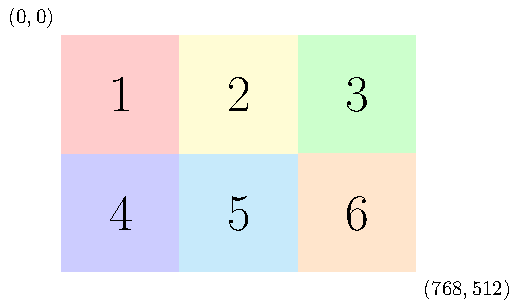
\includegraphics{images/texture.pdf} \end{center}
Supposez que la couleur du pixel de la $i$-ième ligne et $j$-ième colonne est donné par $T[i][j]$ et supposez que vous avez un cube $C$ dont le centre est donné par $C.\Call{centre}{}$ et la demi-longueur d'un côté est $C.\Call{rayon}{}$.
Donnez le pseudocode d'une fonction dont l'en-tête est
\entetefunc{CouleurPixel}{$p$ : point, $C$ : cube, $T$ : texture}{couleur}
qui indique pour chaque point $p$ qui se trouve sur le cube $C$, la couleur du pixel qu'il devrait avoir. Il y a plusieurs solutions possibles à ce problème, mais vous devez respecter les contraintes suivantes~:
\begin{itemize}
  \item Chacun des 6 chiffres doit apparaître sur une face;
  \item Deux faces opposées doivent avoir une somme de $7$.
\end{itemize}
\textbf{Remarque~:} vous n'avez pas à valider si $p$ est bien un point qui se trouve sur le cube, vous pouvez supposer que c'est toujours le cas.
\begin{solution}
	\begin{algorithmic}
	\Function{CouleurPixel}{$p$ : point, $C$ : cube, $T$ : texture} : {couleur}
	\State var $i, j$
	\State $centre \gets \Call{C.Centre}{}$
	\State $rayon \gets \Call{C.Rayon}{}$

	\If 
	{
		$(centre.x - rayon) \leq p.x \leq (centre.x + rayon) \land \newline$
		$\indent (centre.y - rayon) \leq p.y \leq (centre.y + rayon) \land \newline$
		$\indent p.z = (centre.z + rayon)$
	}
		\State $i \gets 0$
		\State $j \gets 0$
	\EndIf

	\If
	{
		$p.x = (centre.x + rayon) \land \newline$
		$\indent (centre.y - rayon) \leq p.y \leq (centre.y + rayon) \land \newline$
		$\indent (centre.z - rayon) \leq p.z \leq (centre.z + rayon)$
	}
		\State $i \gets 0$
		\State $j \gets 1$
	\EndIf

	\If 
	{
		$(centre.x - rayon) \leq p.x \leq (centre.x + rayon) \land \newline$
		$\indent p.y = (centre.y - rayon) \land \newline$
		$\indent (centre.z - rayon) \leq p.z \leq (centre.z + rayon)$
	}
		\State $i \gets 0$
		\State $j \gets 2$
	\EndIf

	\If 
	{
		$(centre.x - rayon) \leq p.x \leq (centre.x + rayon) \land \newline$
		$\indent p.y = (centre.y + rayon) \land \newline$
		$\indent (centre.z - rayon) \leq p.z \leq (centre.z + rayon)$
	}
		\State $i \gets 1$
		\State $j \gets 0$
	\EndIf

	\If 
	{
		$p.x = (centre.x - rayon) \land \newline$
		$\indent (centre.y - rayon) \leq p.y \leq (centre.y + rayon) \land \newline$
		$\indent (centre.z - rayon) \leq p.z \leq (centre.z + rayon)$
	}
		\State $i \gets 1$
		\State $j \gets 1$
	\EndIf

	\If 
	{
		$(centre.x - rayon) \leq p.x \leq (centre.x + rayon) \land \newline$
		$\indent (centre.y - rayon) \leq p.y \leq (centre.y + rayon) \land \newline$
		$\indent p.z = (centre.z - rayon)$
	}
		\State $i \gets 1$
		\State $j \gets 2$
	\EndIf

	\State \textbf{return} \Call{T}{$i, j$}
	\EndFunction
	\end{algorithmic}
\end{solution}

% Trajectoire
\question[15]
Deux objets décrivent une trajectoire rectiligne dans l'espace 3D selon les fonctions vectorielles suivantes~:
\begin{eqnarray*}
  \vec{r_1}(t) & = & (t + 5, 2t - 2, 3t - 1) \\
  \vec{r_2}(t) & = & (3t - 3, 2t - 2, 15 - t),
\end{eqnarray*}
pour $t \geq 0$, où $t$ représente le temps en heures. Est-ce que les trajectoires des objets s'intersectent ? Est-ce que les objets entreront en collision ? Si oui, à quel moment ? Justifiez.
\begin{solution}
On cherche la valeur \emph{t} (si elle existe) pour laquelle les 3 composantes \emph{X, Y} et \emph{Z} des 2 fonctions vectorielles sont égales (collision). Commençons par trouver une valeur de \emph{t} qui satisfait cette condition pour la composante \emph{X}:

\begin{align*} 
t + 5 & = 3t - 3 \\
5 & = 2t - 3 \\ 
8 & = 2t \\ 
4 & = t
\end{align*}

Vérifions maintenant si la composante \emph{Y} des 2 objets est égale pour t = 4 : 

\begin{align*} 
2t - 2 & = 2t - 2 \\
2(4) - 2 & = 2(4) - 2 \\
6 & = 6 \\
\end{align*}

Vérifions maintenant si la composante \emph{Z} des 2 objets est égale pour t = 4 : 

\begin{align*} 
3t - 1 & = 15 - t \\
3(4) - 1 & = 15 - (4) \\
11 & = 11
\end{align*}

Comme la valeur satisfait les 3 composantes, on peut conclure que la collision à bien lieu. Elle survient lorsque t = 4.

\end{solution}

% Lumière
\question[20]
Considérez un cube dont les 8 sommets sont $(\pm 1, \pm 1, 1 \pm 1)$ et qui repose sur le plan $z = 0$. Une source de lumière se trouve en position $(4,4,2)$ et éclaire tout point de l'espace avec la même intensité, peu importe la distance (s'il existe un d'obstacle entre le point et la source de lumière, alors la lumière ne parvient pas au point). Décrivez la forme de l'ombre induite par le cube sur le plan et calculez son aire. \emph{Remarque~:} N'hésitez pas à joindre un schéma de la situation pour mieux expliquer votre réponse.

\begin{solution}
Pour déterminer la forme de l'ombre induite par le cube, on doit tout d'abord trouver l'équation paramétrique définissant le vecteur entre les points L (lumière, voir schéma) et chacun des sommets du cube \emph{qui ne possèdent pas d'obstacle entre leur position, la source lumineuse L et le plan Z}. Ensuite, on détermine la valeur du paramètre lorsque la composante Z vaut 0. En utilisant ce paramètre, on peut trouver les valeurs X et Y du point où le rayon lumineux touche le plan Z, marquant ainsi un des sommets de la forme de l'ombre. Dans le cas présent, on peut considérer que les sommets E,F,G et H font partie de l'ombre puisqu'ils touchent le plan Z. Les sommets A et B du cube ne peuvent pas être considérés, car leur hauteur Z est égale à la hauteur de la source lumineuse ; \emph{une droite passant par la source L et un de ces sommets serait alors parallèle au plan Z}. On doit donc utiliser d'autres points du cube pour estimer la forme de l'ombre. Ici : on a choisi les points $C(-1,1,1)$ et $D(1,-1,1)$. \\ Définissons l'équation paramétrique de la droite passant par L et C d'après le vecteur $\vec{LC}$: 

$\vec{LC} = C - L = ( (-1 - 4) , (1-4) , (1-2) ) = (-5,-3,-1)$\\
$
\left \{
   \begin{array}{r c l}
      X & = & -1 + -5t \\
      Y & = & 1 + -3t \\
      Z & = & 1 + -t
   \end{array}
\right .
$\\
On doit maintenant trouver la valeur de $t$ pour laquelle la droite croise le plan, i.e : lorsque $Z = 0$ : 

\begin{align*} 
0 & = 1 - t \\
-1 & = -t \\ 
1 & = t 
\end{align*}
\newline
On remplace alors cette valeur de $t$ pour trouver la valeur des autres composantes : 
$
\left \{
   \begin{array}{r c l}
      X & = & -1 + -5(1) = -6\\
      Y & = & 1 + -3(1) =  -2
   \end{array}
\right .
$\\
\newpage
Il nous reste à faire la même chose avec le vecteur $\vec{LD}$: 

$\vec{LD} = D - L = ( (1 - 4) , (-1-4) , (1-2) ) = (-3,-5,-1)$\\
$
\left \{
   \begin{array}{r c l}
      X & = & 1 + -3t \\
      Y & = & 1 + -5t \\
      Z & = & 1 + -t
   \end{array}
\right .
$\\
La valeur de $t$ lorsque $z = 0$ est la même que précédemment.
On remplace alors cette valeur de $t$ pour trouver la valeur des autres composantes : \\
$
\left \{
   \begin{array}{r c l}
      X & = & -1 + -3(1) = -2\\
      Y & = & 1 + -5(1) =  -6
   \end{array}
\right .
$\\
Le schéma suivant montre la forme qu'aura l'ombre. Il n'est pas possible de donner l'air de cette forme, car 2 des points qui la constituent ont leur position à des distances infinies.

\begin{center} 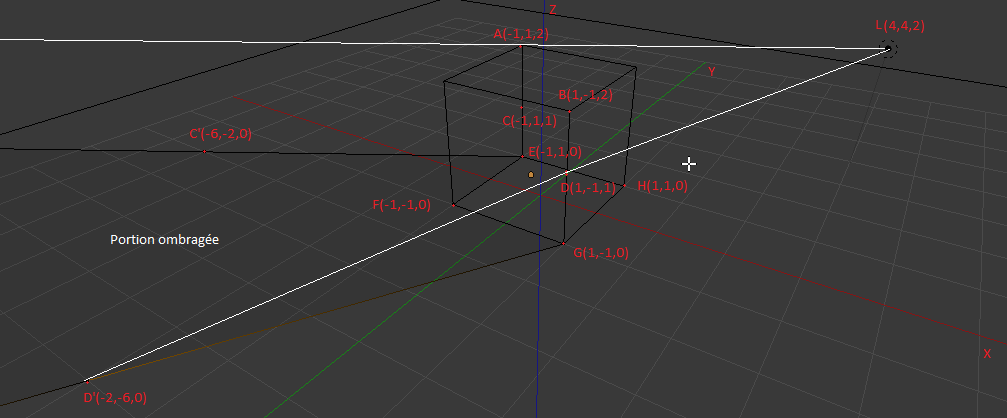
\includegraphics[width=1\linewidth]{images/q5.png} \end{center}
\end{solution}

\end{questions}

\end{document}
